% manfra comments:
%         didn't understand how the measurement was done. thought we were measuring Vmid and seeing it shift.  
%         wanted to know more about how this technique would actually be implemented to realize one of the more exciting proposals.

% mohammad comments:
% 	    Figure 2 -- (c) make more clear how delta T was obtained
%         make more clear how the 5/2 measurement relates to what was done here
%         gate-tuned -- change this phrase in the methods
%         I_heat looks like it shorts the sample in Figure 1a
%         Nature Methods -- suggestion for journal

\documentclass[twocolumn,showpacs,amsmath,amssymb,prl,aps,superscriptaddress]{revtex4-1}

\usepackage{graphicx}
\usepackage{amsmath}
\usepackage{siunitx}
\usepackage{hyperref}

\newcommand{\ket}[1]{\ensuremath{\left|#1\right\rangle}}

\begin{document}

\title{Direct Entropy Measurement in a Mesoscopic Quantum System}
\author{Nikolaus Hartman}
\email{nik.hartman@gmail.com}
\thanks{The raw data and Python code used for all figures and analysis can be found at \url{https://github.com/nikhartman/spin_entropy}}
	\affiliation{Stewart Blusson Quantum Matter Institute, University of British Columbia, Vancouver, British Columbia, V6T1Z4, Canada}
	\affiliation{Department of Physics and Astronomy, University of British Columbia, Vancouver, British Columbia, V6T1Z1, Canada}
\author{Christian Olsen}
	\affiliation{Stewart Blusson Quantum Matter Institute, University of British Columbia, Vancouver, British Columbia, V6T1Z4, Canada}
	\affiliation{Department of Physics and Astronomy, University of British Columbia, Vancouver, British Columbia, V6T1Z1, Canada}
\author{Silvia Folk}
	\affiliation{Stewart Blusson Quantum Matter Institute, University of British Columbia, Vancouver, British Columbia, V6T1Z4, Canada}
	\affiliation{Department of Physics and Astronomy, University of British Columbia, Vancouver, British Columbia, V6T1Z1, Canada}
\author{Mohammad Samani}
	\altaffiliation{The Hospital for Sick Children, Toronto, ON, Canada}
	\altaffiliation{Fields Institute for Research in Mathematical Sciences, Toronto, ON, Canada}
	\affiliation{Stewart Blusson Quantum Matter Institute, University of British Columbia, Vancouver, British Columbia, V6T1Z4, Canada}
	\affiliation{Department of Physics and Astronomy, University of British Columbia, Vancouver, British Columbia, V6T1Z1, Canada}
\author{Saeed Fallahi}
	\affiliation{Department of Physics and Astronomy, Purdue University, West Lafayette, Indiana, USA}
	\affiliation{Station Q Purdue, Purdue University, West Lafayette, Indiana, USA}
	\affiliation{Birck Nanotechnology Center, Purdue University, West Lafayette, Indiana, USA}
\author{Geoffrey C. Gardner}
	\affiliation{Station Q Purdue, Purdue University, West Lafayette, Indiana, USA}
	\affiliation{Birck Nanotechnology Center, Purdue University, West Lafayette, Indiana, USA}
    	\affiliation{School of Materials Engineering, Purdue University, West Lafayette, Indiana, USA}
\author{Michael Manfra}
	\affiliation{Department of Physics and Astronomy, Purdue University, West Lafayette, Indiana, USA}
	\affiliation{Station Q Purdue, Purdue University, West Lafayette, Indiana, USA}
	\affiliation{Birck Nanotechnology Center, Purdue University, West Lafayette, Indiana, USA}
	\affiliation{School of Electrical and Computer Engineering,  Purdue University, West Lafayette, Indiana, USA}
    	\affiliation{School of Materials Engineering, Purdue University, West Lafayette, Indiana, USA}
\author{Joshua Folk}
\email{jfolk@physics.ubc.ca}
	\affiliation{Stewart Blusson Quantum Matter Institute, University of British Columbia, Vancouver, British Columbia, V6T1Z4, Canada}
	\affiliation{Department of Physics and Astronomy, University of British Columbia, Vancouver, British Columbia, V6T1Z1, Canada}
\date{\today}

\maketitle

%%%%%%% intro material %%%%%%%%%
\textbf{The thermodynamic properties of electronic systems offer important insights into the nature of their ground states, and can probe exotic quasiparticles that may emerge due to interactions or non-trivial topology.  Systems that are difficult to clearly identify through standard conductance measurements may be characterized more precisely with a thermodynamic measurement. For example, the purported non-Abelian exchange statistics of Moore-Read quasiparticles in the $\nu = \frac{5}{2}$ fractional quantum Hall state, or of Majorana quasiparticles in a topological superconductor, could be clearly distinguished from the Abelian case by an entropy measurement \cite{Cooper2009, Ben-Shach2013, Smirnov2015}.  
Such measurements are typically based on bulk properties, like heat capacity, that are easily observed in macroscopic samples but are immeasurably small in systems that may consist of only a few electrons.  Here, we develop a mesoscopic circuit to make direct entropy measurements of single- or few-quasiparticle states---in this case, the first, second, and third electron ground states in a GaAs quantum dot.  This system is chosen for having well-known entropy based on simple spin states\cite{Tarucha1996, Ciorga2000, Duncan2000, Lindemann2002, Potok2003, Hofmann2016}.  The precision of this technique, quantifying the entropy of a single spin-$\frac{1}{2}$ to within 5\% of the expected value ($k_B \ln{2}$), shows its future potential for probing more exotic systems, from Majorana states to non-Fermi liquid Kondo states, that are clearly identified by their residual low-temperature entropy\cite{Alkurtass2016}.}

%%% figure 1 %%%
\begin{figure}[!]
        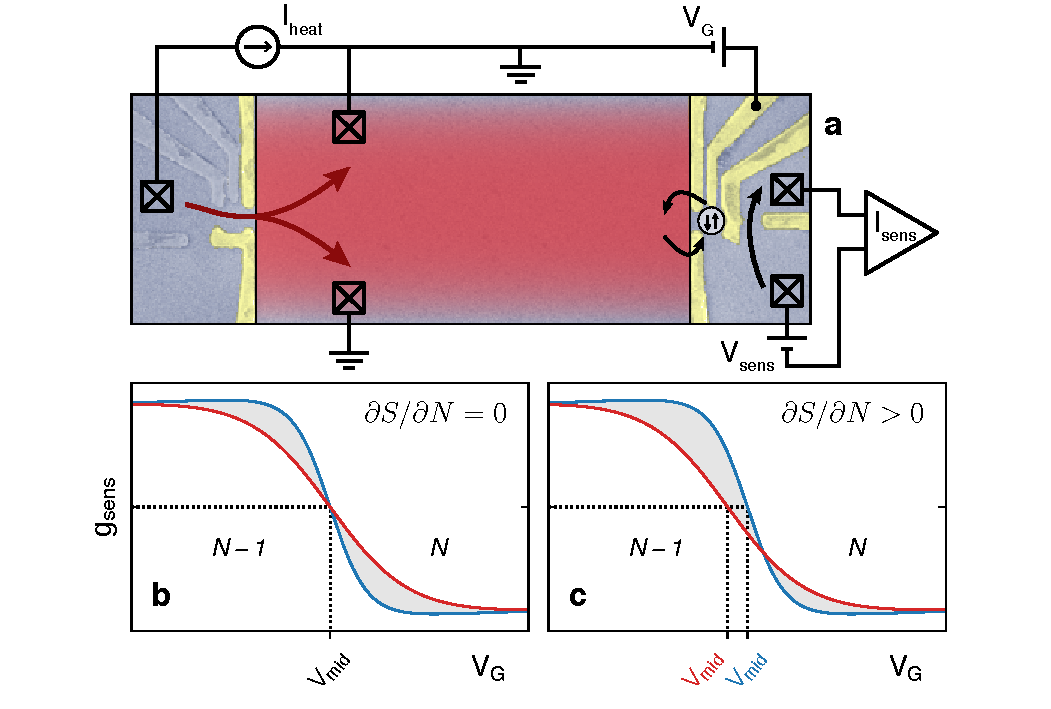
\includegraphics[width=1.0\columnwidth]{../figures/figure_1_annotated.pdf}
        \caption{\label{fig:fig1} \textbf{Entropy measurement protocol.}  (a) Scanning electron micrograph of a device similar to the one measured. Electrostatic gates (gold) define the circuit in a 2D electron gas (2DEG), with grey gates grounded. Squares indicate ohmic contacts to the 2DEG.  The temperature of the electron reservoir in the middle (red) is oscillated using AC current, $I_{heat}$, at frequency $f_{heat}$ through the quantum point contact (QPC) on the left.  A portion of the $5~\mu$m-wide reservoir has been removed here for clarity.  The occupation of the quantum dot, tunnel coupled to the right side the reservoir, is tuned by $V_p$ and monitored by $I_{sens}$ through the charge sensor QPC. $I_{sens}$ is split into DC and AC components, the latter being measured by a lock-in amplifier at $2f_{heat}$.  (b) and (c) Simulated DC charge sensor signal, $G_{sens}$, for a transition from $N-1 \rightarrow N$ electrons at two temperatures ($T_{Red} > T_{Blue}$), showing two possible cases for $\frac{\partial S}{\partial N}$. Insets show the corresponding difference, $\delta G_{sens}$, between hot and cold curves.}
\end{figure}

Our approach is analogous to the milestone of spin-to-charge conversion achieved over a decade ago, in which the infinitesimal magnetic moments of a single spin were detected by transforming them into the presence or absence of an electron charge \cite{Elzerman2004, Ono2004}.  Following this logic, we perform an entropy-to-charge conversion, making use of the Maxwell relation
%
\begin{align}
\label{eqn:max}
        \left(\frac{\partial \mu}{\partial T}\right)_{p,N} &= -\left(\frac{\partial S}{\partial N}\right)_{p,T}
\end{align}
%
that connects changes in entropy, particle number, and temperature ($S$, $N$, and $T$, respectively) to changes in the chemical potential, $\mu$, a quantity that is simple to measure and control. The fixed pressure condition of Eq.~\ref{eqn:max} is met by working well below the Fermi temperature of the 2DEG, $T_F \sim \SI{5}{\kelvin}$, where degeneracy pressure dominates \cite{Landau1969}.

The Maxwell relation in Eq.~\ref{eqn:max} forms the basis of two theoretical proposals to measure non-Abelian exchange of quasiparticles in  the $\nu = \frac{5}{2}$ state via their entropy
%, quantified by the change in quasiparticle chemical potential with temperature
\cite{Cooper2009,Ben-Shach2013}.  Ref.~\onlinecite{Ben-Shach2013} proposes a strategy by which quasiparticle entropy could be deduced from the temperature-dependent shift of charging events on a local disorder potential, a thermodynamic equivalent of the measurements that established the $e/4$ quasiparticle charge\cite{Venkatachalam2011}.   As a proof of principle in the viability of measuring localized quasiparticle entropy, and a demonstration of the high accuracy achievable by this technique, we investigate a well-understood system with localized fermions: a few-electron GaAs quantum dot. The entropies of the first three electron states in the dot are measured by the temperature-dependent charging scheme laid out in Ref.~\onlinecite{Ben-Shach2013}.   Applying the language of quantum dots to Eq.~\ref{eqn:max}, the entropy difference between the $N-1$ and $N$ electron ground states ($\Delta S_{N-1\rightarrow N}$ for $\Delta N=1$) is measured via the shift with temperature in the electrochemical potential, $\mu_N$, needed to add the $N$th electron to the dot. 

The measurement relies on the mesoscopic circuit shown in Fig.~\ref{fig:fig1}a, using electrostatic gates to realize an electron reservoir (hereafter ``reservoir") in thermal and diffusive equilibrium with a few-electron quantum dot (``dot") coupled to its right side.  The occupation of the dot is tuned with the plunger gate voltage, $V_p$, and measured using an adjacent quantum point contact (``charge sensor") \cite{Field1993, Staring2007, Thierschmann2015}.  Applying more positive $V_p$ lowers $\mu_N$,  bringing the $N$th electron into the dot when $\mu_{N}$ drops below the Fermi level of the reservoir, $E_F$. The reservoir temperature, $T$, can be increased above the mixing chamber temperature, $T_{MC}$, by Joule heating from current $I_{heat}$ through the quantum point contact (``heater") on the left side.   Charge transitions on the dot appear as steps in the charge sensor conductance, $G_{sens}(V_p)$, thermally broadened by the reservoir temperature (Figs.~\ref{fig:fig1}b and c).  The gate voltage corresponding to the midpoint of the transition, $V_{mid}$, marks the electrochemical potential at which the probabilities of finding $N-1$ and $N$ electrons on the dot are equal.

When $\mu_N$ shifts with temperature (Eq.~\ref{eqn:max}), $V_{mid}$ also shifts; it is the shift in $V_{mid}$ with temperature that forms the basis of our experiment (Fig.~\ref{fig:fig1}c).  In practice, charge noise limits the accuracy to which $V_{mid}$ can be measured, so the measurement is done with a lock-in amplifier, oscillating the temperature using an AC $I_{heat}$ and measuring resultant oscillations in $G_{sens}$.  As seen in the insets of Figs.~\ref{fig:fig1}b and c, the lineshape of $\delta G_{sens}$ is perfectly antisymmetric when $\partial S/\partial N=0$, but asymmetric when $\partial S/\partial N \neq 0$.

The temperature-induced shift in the dot chemical potential with respect to reservoir $E_F$ can also be understood in terms of detailed balance.  At $V_{mid}$, with equal probabilities for $N$ and $N-1$ electrons on the dot, the tunnel rates $\Gamma_{in}=\Gamma_{N-1\rightarrow N}$ and $\Gamma_{out}=\Gamma_{N\rightarrow N-1}$ must also be equal. These rates depend on the number of available states in the tunneling process, and therefore on the degeneracies of the $N-1$ and $N$ ground states \cite{Beenakker1991, Gustavsson2009}.  The condition $\Gamma_{in} = \Gamma_{out}$ leads to a simple relationship between the degeneracies, $d_{N-1}$ and $d_{N}, of the $N-1$ and $N$ electron states and the thermally broadened Fermi function $f$: $d_{N-1}/d_{N}=f/(1-f)$. Using the Boltzman entropy, $S_{N}=k_{B} \ln{d_N}$, and the form of the Fermi function, this relationship becomes $\Delta S_{N-1\rightarrow N}= (\mu_{N}-E_F)/T$, clearly demonstrating the connection between entropy, temperature, and the shift in $\mu_N$ relative to $E_F$ at $V_{mid}$. Previous experiments have explored the relationship between tunnel rates and degeneracy using time-resolved transport spectroscopy and by coupling quantum dots to atomic force cantilever oscillations \cite{Cockins2010, Bennett2010, Beckel2014, Hofmann2016}. The approach presented here is a thermodynamic equivalent of these, and extends entropy measurements to a much wider set of applications where tunnelling processes may not be possible to observe in real-time.

%%% figure 2 %%%
\begin{figure}[!]
        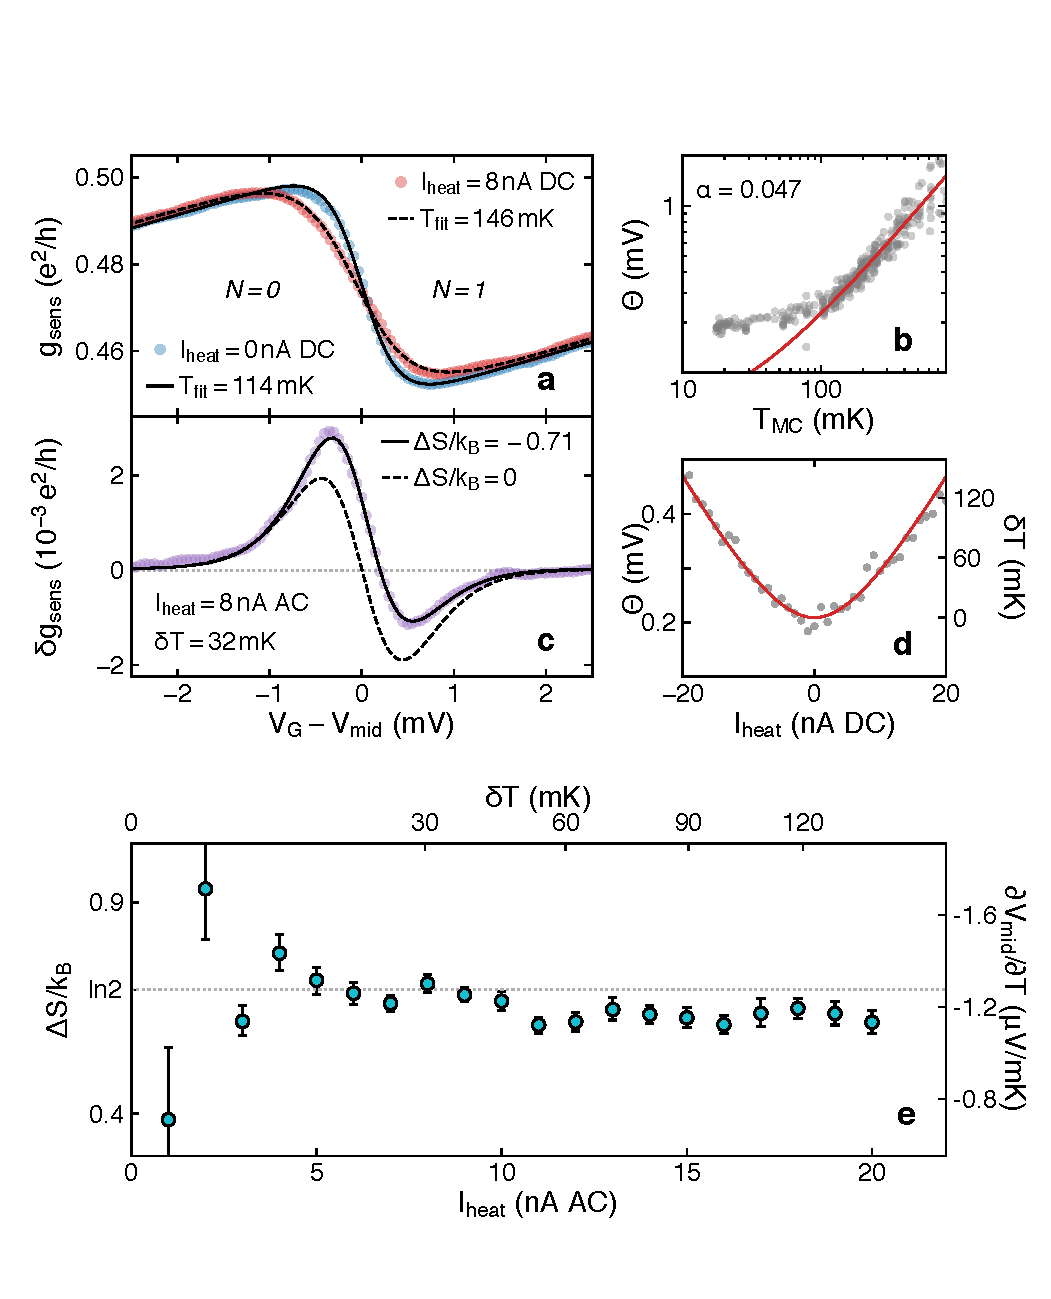
\includegraphics[width=1.0\columnwidth]{../figures/figure_2.pdf}
        \caption{\label{fig:fig2} \textbf{Entropy measurement for a single spin $\frac{1}{2}$.} (a) Charge sensor data for $N=0 \rightarrow 1$ at two temperatures set by DC current through the QPC heater. (b) Transition width, $\Theta$, was linear in $T_{MC}$ above 100 mK, for $I_{heat}=0$. Lever arm $\alpha$ is calculated by fitting a straight line to this region.  (c) Lock-in measurement of $\delta G_{sens}$ with $\delta T = \SI{32}{\milli\kelvin}$, determined from the calibration in panel (d). Fits to $\delta G_{sens}$ (Eq.~\ref{eqn:dg-sens}) are shown with $\Delta S / k_B$  as a free parameter (solid) and fixed at $\Delta S / k_B=0$ (dashed). (d) $\Theta$ grows with DC current through the QPC heater. A fit to $T = a\sqrt{T^{2}_{MC}+b I^2_{heat}R_{QPC}}$ is used to convert between $I_{heat}$ and $\delta T$\cite{Mittal1996}. (e)  Entropy measurements were independent of the magnitude of $I_{heat}$ oscillations over a large range. The top axis indicates the corresponding magnitude of $\delta T$, while the right axis shows the entropy signal converted to a gate voltage shift per unit temperature.}
\end{figure}

%To proceed with the entropy measurement,
The dot was tuned such that the source was weakly tunnel coupled to the reservoir with the drain closed.  The conductance of the charge sensor was tuned to $G_{sens}{\sim}e^2/h$, where it was most sensitive to charge on the dot.  The addition of the first electron to the dot was marked by a decrease in $G_{sens}$ that is well described as a thermally-broadened two-level transition (Fig.~\ref{fig:fig2}a):
%
\begin{align}
\label{eqn:g-sens}
        G_{sens}(V_p,\Theta) &= G_0 \tanh\left(\frac{V_p - V_{mid}(\Theta)}{2\Theta}\right)  \\
                        &\quad + G_1 V_{G} + G_2 \nonumber
\end{align}
%
where $G_0$ quantifies the sensor sensitivity, $\Theta = \frac{k_B T}{\alpha e}$ is the thermal broadening (expressed in units of gate voltage), $\alpha\equiv d \mu_{N}/d V_p$ is the lever arm,  $G_1$ reflects the cross capacitance between the charge sensor and plunger gate, and $G_2$ is an offset. Figure~\ref{fig:fig2}a shows two such transition curves with thermal broadening set by the current, $I_{heat}$ through the heater. For $I_{heat}=0$, $\Theta$ followed $T_{MC}$ down to \SI{<100}{\milli\kelvin} (Fig.~\ref{fig:fig2}b), validating the approximation of thermal broadening used throughout this experiment.

The data in Fig.~\ref{fig:fig2}c, and corresponding fits, illustrate a measurement of $\Delta S_{0\rightarrow 1}$ across the $0 \rightarrow 1$ electron transition. The lock-in measurement of $\delta G_{sens}$ due to temperature oscillations $\delta T$ yields the characteristic peak-dip structure seen in Fig.~\ref{fig:fig2}c, corresponding the difference between the two $G_{sens}$ curves in Fig.~\ref{fig:fig2}a. The expected lineshape of such a curve is $\delta G_{sens} = \frac{\partial G_{sens}}{\partial T} \delta T$, with $G_{sens}$ defined by Eq. \ref{eqn:g-sens}.  This lineshape depends in a simple way on $\Delta S$, recognizing (via Eq.~\ref{eqn:max}) that $\frac{\partial V_{mid}}{\partial \Theta}=\frac{1}{k_B}\frac{\partial \mu}{\partial T} =\frac{1}{k_B}\Delta S_{N-1\rightarrow N}$:
%
\begin{align}
\label{eqn:dg-sens}
        \delta G_{sens}(V_p, \Theta) &\propto -\delta T \left[ \frac{V_p - V_{mid}(\Theta)}{2\Theta} - \frac{\Delta S}{2k_B} \right]\times \\
        				      &\quad\cosh^{-2}\left(\frac{V_p - V_{mid}(\Theta)}{2\Theta}\right) + const. \nonumber
\end{align}
%


\noindent As expected  from Figs.~\ref{fig:fig1}b,c, $\delta G_{sens}(V_p)$ is antisymmetric around $V_{mid}$ for $\Delta S=0$, and asymmetric for $\Delta S\neq 0$.  A fit of the data in Fig.~\ref{fig:fig2}c to Eq.~\ref{eqn:dg-sens} yields $\Delta S_{0\rightarrow 1}=(1.02 \pm 0.03) k_B \ln{2}$, closely matching the expected $\Delta S_{0 \rightarrow 1} = S_1 - S_0 =k_B\ln{2}$ for transitions between an empty dot ($S_0=0$) and the two-fold degenerate 1-electron state ($d_1=2$) with entropy $S_1=k_B \ln{2}$.

It is important to note that extracting $\Delta S$ from fits to Eq.~\ref{eqn:dg-sens} can be done just from the asymmetry of the lineshape, with no calibration of measurement parameters (such as $\delta T$ or the lever arm $\alpha$) required.  We can, however, estimate $\delta T$ and $\alpha$ by measuring $T(I_{heat})$, using a DC $I_{heat}$ to raise the reservoir temperature and fitting to Eq.~\ref{eqn:g-sens}  (Fig.~\ref{fig:fig2}d); the calibration holds for AC currents below 100 Hz.  Measurements of $\Delta S$ remained constant over a broad range of $\delta T$ (Fig.~\ref{fig:fig2}e), as expected for temperatures low enough not to excite orbital degrees of freedom on the dot. 

%%% figure 3 %%%
\begin{figure}
        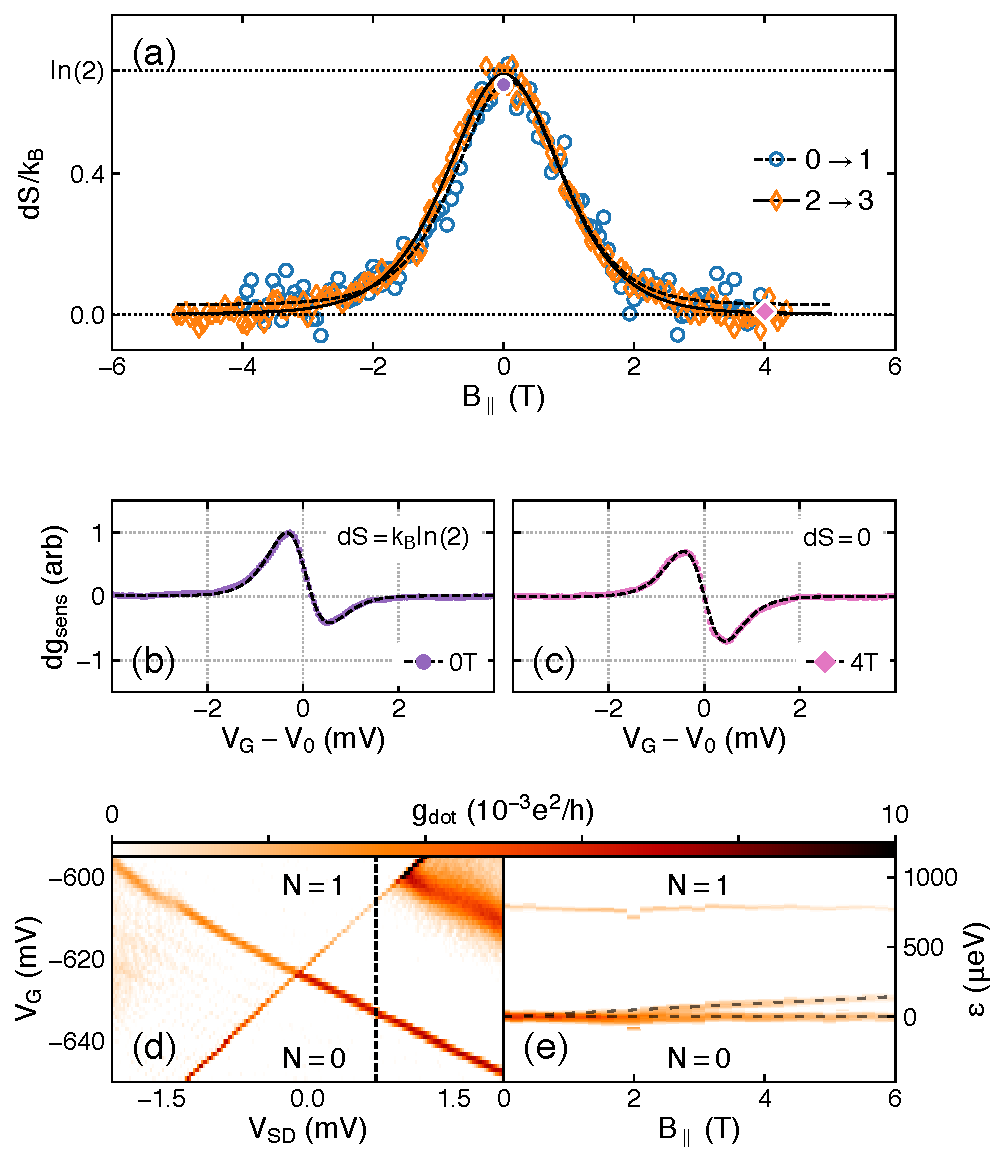
\includegraphics[width=1.0\columnwidth]{../figures/figure_3.pdf}
        \caption{\label{fig:fig3} \textbf{Magnetic field dependence.} (a) Changes in entropy for $N=0 \rightarrow 1$ and $2 \rightarrow 3$ transitions, overlaid to highlight similar behaviors.  Each data point corresponds to a single $\delta G_{sens}(V_p)$ fit; multiple scans are carried out at various parallel magnetic fields.   (b) and (c) Characteristic $\delta G_{sens}$ traces from which the data in (a) were extracted. The two data points corresponding to (b) and (c) are shown as large markers in (a). (e) Bias spectroscopy data for the $N=0 \rightarrow 1$ transition. Dashed line at $V_{SD}$ = \SI{700}{\micro\electronvolt} shows where data in (f) are taken. (f) Fixed bias data showing fits to Zeeman splitting of the ground state (dashed lines) from which $g = -0.42 \pm 0.01$ is extracted.}
\end{figure}

Confirmation that the measured $\Delta S$ derives from spin degeneracy is seen through its evolution with in-plane magnetic field, $B_\parallel$. Figure \ref{fig:fig3}a compares $\Delta S(B_\parallel)$ for the $0 \rightarrow1 $ and $2 \rightarrow 3$ transitions, both of which correspond to transitions from total spin zero to total spin one-half. The entropies of the $\ket{S=1/2}$ states go to zero as when Zeeman splitting lifts the spin degeneracy, given by the Gibbs entropy for a two-level system:
%
\begin{align}
\label{eqn:gibbs}
        S &= k_B \sum_{i=\pm} p_{i}(B_\parallel, T) \ln{ p_{i}(B_\parallel,T) }
\end{align}
%
where $p_{\pm}(B_\parallel, T) = (1+ e^{\mp \frac{g\mu_B B_{\parallel}}{k_B T}})^{-1}$ are the probabilities for the unpaired electron to be in the spin up/down states at a given field and temperature. Fits to Eq.~\ref{eqn:gibbs}, with the ratio $g/T$ and an added scaling $\Delta S(B=0)$ as free parameters, give $\Delta S_{0 \rightarrow 1}(B=0)=(0.94 \pm 0.03) k_B \ln{2}$ and $\Delta S_{2 \rightarrow 3}(B=0)=(0.98 \pm 0.02) k_B \ln{2}$ (Fig.~\ref{fig:fig3}), and reflect the collapse to zero at high field where spin degeneracy is broken. This collapse can also be seen qualitatively, as a crossover from asymmetric to antisymmetric lineshapes for $\delta G_{sens}(V_p)$ (Figs.~\ref{fig:fig3}b and c). Estimating an average $T$ for each data set using the calibration in Fig.~\ref{fig:fig2}d yields $|g|=0.48 \pm 0.02$ and $|g|=0.44 \pm 0.01 $ for the $0\rightarrow 1$ and $2\rightarrow 3$ transitions, respectively. Errors in the g-factor measurement are likely due to the difficulty of estimating temperature oscillations. Still, the g-factors are consistent with reported values\cite{Cronenwett1998,Hanson2003,Zumbuhl2004} and the value measured separately in Fig.~\ref{fig:fig3}e using bias spectroscopy.

%%% figure 4 %%%
\begin{figure}
        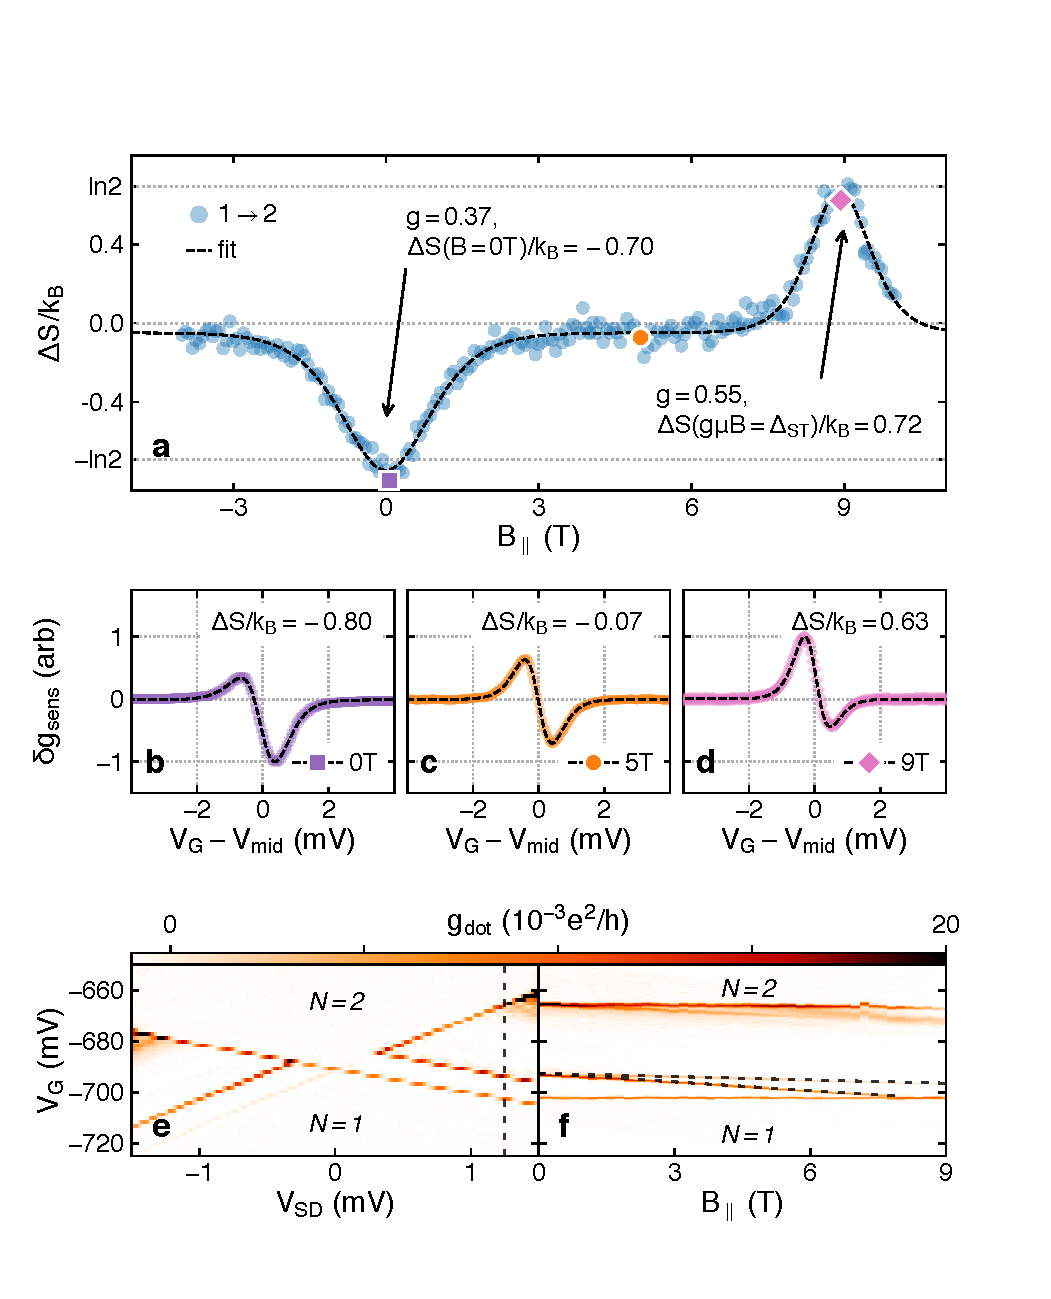
\includegraphics[width=1.0\columnwidth]{../figures/figure_4.pdf}
        \caption{\label{fig:fig4}  \textbf{Entropic signature of a singlet-triplet crossing.} (a) Change in entropy, extracted from $\delta G_{sens}$ fits at varying parallel field. Dashed line shows fit to Eq.~\ref{eqn:gibbs}. Values stated for $\Delta S$ are with respect to the vertical offset apparent in the data. (b), (c), and (d) show characteristic $\delta G_{sens}$ traces from which the data in (a) were extracted. These data points are show as large markers in (a). (e) Bias spectroscopy data for the $N=1 \rightarrow 2$ transition. Transitions to the 2-electron triplet state correspond to the lines appearing at $V_{SD} = \SI{\pm 320}{\micro\electronvolt}$. Dashed line at $V_{SD}$ = \SI{1250}{\micro\electronvolt} shows where data in (f) are taken. (f) Fixed bias data in parallel field. Triplet level is split into $\ket{T_+}$ and $\ket{T_0}$ levels with a third $\ket{T_-}$ level not visible here. At \SI{8.4}{\tesla} $\ket{T_+}$ becomes degenerate with $\ket{S}$. $g=-0.40\pm0.04$ is determined using $\ket{T_0}$ and $\ket{T_+}$ fits (dashed).}
\end{figure}

The $1\rightarrow 2$ transition can be understood as the inverse of the $0 \rightarrow 1$ transition for $B_\parallel < \SI{5}{\tesla}$, comparing Figs~\ref{fig:fig3}a and \ref{fig:fig4}a. For relatively low fields, the 2-electron ground state remains a spin singlet ($\ket{S=0}$) with zero entropy, while the 1-electron entropy goes from $k_B\ln{2}$ to zero due to Zeeman splitting.  At higher fields, the 1-electron ground state remains non-degenerate while the 2-electron ground state gains a two-fold degeneracy when the singlet and triplet \ket{T_+} states cross.  This singlet-triplet crossing is seen in bias spectroscopy data (Fig.~\ref{fig:fig4}f) at \SI{8.4}{\tesla}, and in the appearance of a peak in $\Delta S_{1\rightarrow 2}$ at \SI{9}{\tesla}.  The discrepancy between the fields required to drive the singlet-triplet degeneracy in Figs.~\ref{fig:fig4}a and f can be explained by the change in dot configuration from one to two open tunnel barriers.

The field-dependent entropy measurement for the $1 \rightarrow 2$ transition can again be fit using Eq.~\ref{eqn:gibbs}, with probabilities as before for the 1-electron states and $p_{\ket{S}/\ket{T}}(B_\parallel, T) = (1+ e^{\mp \frac{g\mu_B B_\parallel - \Delta_{ST}}{k_B T}})^{-1}$ for the 2-electron states, where $\Delta_{ST}$ is the singlet-triplet splitting at zero field. The fit in Fig.~\ref{fig:fig4}a allows for an offset from $\Delta S=0$ away from the degenerate points to compensate for non-linearities in the charge sensor. From the fit, we find $\Delta S_{1\rightarrow 2}$ at the two-fold degenerate points, $B=0$ and \SI{9}{\tesla}, are $-(1.01\pm0.03) k_B \ln{2}$ and $(1.04 \pm 0.04) k_B \ln{2}$, respectively. The extracted g-factor, $g = 0.47 \pm 0.02$, from the peak at $B=0$ is consistent with the $0\rightarrow 1$ transition.  At the high-field singlet-triplet degeneracy we find $g = 0.69 \pm 0.04$, an unexpectedly high g-factor that may be explained by a shift of the $\ket{T_0}$ state with magnetic field, as seen in Fig.~\ref{fig:fig4}f and previous work \cite{Szafran2004}.  The high quality of the Gibbs entropy fit, over a large range of field, confirms that the measured signal is the change in entropy $\Delta S$, and illustrates a tuneable degeneracy.

%%% conclusion %%%
%In conclusion, we have presented a direct entropy measurement of the few-particle states in a few electron states in a GaAs was quantified within 5\% of the expected $k_B \ln{2}$.  Future work may take advantage of this strategy to search for thermodynamic signatures of quantum states with non-trival correlations or topology, eliminating the uncertainty found in typical transport data.

\paragraph*{Methods} The device was built on a AlGaAs/GaAs heterostructure, hosting a 2D electron gas with density and mobility at \SI{300}{\milli\kelvin} (determined in a separate chip/measurement) of \SI{2.42e11}{\per\square\centi\metre} and \SI[per-mode=symbol]{2.56e6}{\square\centi\metre\per\volt\per\second} respectively.   Mesas and NiAuGe ohmic contacts to the 2DEG were defined by standard photolithography techniques, followed by atomic layer deposition of \SI{10}{\nano\metre} $\mathrm{HfO_2}$ to improve the gating stability in the device. Fine gate structures, shown in Fig.~\ref{fig:fig1}a, were defined by electron beam lithography and deposition of \SI{3/18}{\nano\metre} Ti/Au. 

The measurement was carried out in a dilution refrigerator with a two-axis magnet. The 2DEG was aligned parallel to the main axis with the second axis used to compensate for sample misalignment. In practice, perpendicular fields up to \SI{100}{\milli\tesla} showed no effect on our data. [ADD DESCRIPTION OF THE CHANGE OF CONFIGURATION FOR BIAS SPECTROSCOPY, AND DETAILS OF SETTINGS FOR ENTROPY MEASUREMENT]  Charge sensor conductance was measured using a DC voltage bias of \SI{200}{\micro\volt}, with the current, measured at DC ($I_{sens}$) using an analog-digital convertor and at AC ($\delta I_{sens}$) using a lock-in amplifier. The DC conductance reported here is $G_{sens}=I_{sens}/V_{sens}$ while $\delta G_{sens}$ is $G_{sens}=(\delta I_{sens})/V_{sens}$.

The temperature of the reservoir could be raised above $T_{MC}$ using $I_{heat}$ at AC or DC, with the heater set by gate voltages to \SI{20}{\kilo\ohm}. Applying AC current at $f_{heat} =$ \SI{48.7}{\hertz} yields an oscillating Joule power, $P_{heat} = I^2_{heat}R_{QPC}$. To leading order this gives oscillations in temperature, and therefore $\delta G_{sens}$, at $2f_{heat}$.  These are  captured by the lock-in amplifier at the second harmonic of $I_{heat}$.  Except where noted, measurements of $\Delta S$ were made at $\delta T \sim $ \SI{50}{\milli\kelvin}, although the error bars in Fig.~\ref{fig:fig2} demonstrate that the measurements would have been just as accurate with $\delta T$ set to \SI{30}{\milli\kelvin}.

%The transition width, $\Theta$, extracted from fits to Eq.~\ref{eqn:g-sens} was found to follow the mixing chamber temperature, $T_{MC}$, to \SI{<100}{\milli\kelvin} (Fig.~\ref{fig:fig2}b). The assumption of thermally broadened transitions greatly simplifies the data analysis, so $T_{MC}$ is fixed at \SI{100}{\milli\kelvin} for most of this work, using Joule heating to raise $T$ up to \SI{250}{\milli\kelvin}. 

\acknowledgments
The authors acknowledge John Martinis for a helpful discussion on the interpretation of our measurements.

\bibliography{qdentropy}{}
\bibliographystyle{apsrev4-1}

\end{document}

%%% old abstract %%%

%\begin{abstract}
%
%Measuring the entropy of an electronic state is a powerful tool for identifying its underlying microscopic character.  Such measurements are typically based on bulk properties, such as heat capacity, that are straightforward to observe in macroscopic samples but exceedingly difficult to access in mesoscopic systems that may consist of just a few electrons. Taking advantage of a well-known Maxwell relation, we realize a protocol for entropy-to-charge conversation in a gate-defined GaAs quantum dot that enables an entropy measurement of the first three quantum states in to the dot. The entropy of a single spin ($k_B \ln{2}$) is measured within 8\% accuracy, as is the entropy arising at the magnetic field-driven singlet-triplet crossing for two electrons.
%
%\end{abstract}

%%% old sentences %%%

%Similarly, the two-channel Kondo state that is believed to arise in carefully tuned GaAs devices has so far been identified through a particular temperature dependence in the device conductance \cite{Potok2007}. A more direct test for the two-channel Kondo state would be a confirmation of its entropy ($\frac{1}{2} k_B \ln{2}$), that should remain down to arbitrarily low temperatures \cite{Alkurtass2016}.

%Entropy can be probed effectively in 3D macroscopic samples via measurements of heat capacity, but the heat capacities of single electrons or quasiparticles are much too small to measure directly; even the 2D sheet of quasiparticles in $\nu = \frac{5}{2}$ fractional quantum Hall samples has a heat capacity that vanishes in comparison to that of the host crystal.  Rather than attempt to resolve such infinitesimal signals, the problem can be avoided by converting changes in entropy to changes in charge \textemdash a quantity that is easily detected at the single particle level.

%Unlike the $\nu = \frac{5}{2}$ quasiparticles described in the theoretical work, the few-electron quantum dot states investigated here have an entropy that is well-understood from the spin degree of freedom \cite{Tarucha1996, Ciorga2000, Duncan2000, Lindemann2002, Potok2003, Hofmann2016}.  

%This shift, $\delta \mu$ as a function of $\delta T$, is the quantity probed directly in the experiment described below. From these measurements the entropies of the first three quantum dot levels are built up, demonstrating a direct entropy measurement is possible on a few-particle system. In the future, the method can be utilized to probe the nature of more exotic systems, such as topologically non-trivial Majorana and other non-Abelian states. 

%Consider the filling of the first electron state, which has a single, unpaired spin-$\frac{1}{2}$ and, therefore, a degeneracy of 2.

%One expects identical field-dependent behaviors for $\Delta S_{0\rightarrow 1}$ and $\Delta S_{2\rightarrow 3}$ as long as $g \mu_{B} B_\parallel$ is less than the excited state energies

%The transition width, $\Theta$, extracted from fits to Eq.~\ref{eqn:g} follows the mixing chamber temperature, $T_{MC}$, to \SI{<100}{\milli\kelvin} (Fig.~\ref{fig:fig2}b). The assumption of thermally broadened transitions greatly simplifies the data analysis, so $T_{MC}$ is fixed at \SI{100}{\milli\kelvin} for most of this work, using Joule heating to raise $T$ up to \SI{250}{\milli\kelvin}. Measurements of $\Delta S$ are made at $\delta T = $ \SI{60}{\milli\kelvin} such that no orbital levels above the ground state were excited.

%Although the extracted $\Delta S / k_B$ can be converted to gate-voltage-per-temperature units using a value for $\alpha$ measured separately (right axis of Fig.~\ref{fig:fig2}e), the entropy itself, $\Delta S$, is determined directly from the fit to $\delta G_{sens}$ without any additional calibration, and without knowing the precise value of $\delta T$.

%
% \begin{align}
% \label{eqn:epsilon}
%         \epsilon &= \frac{\partial V_{mid}}{\partial \Theta} = 
%         \frac{1}{k_B} \frac{\partial \mu}{\partial T} = 
%         -\frac{1}{k_B} \Delta S_{N-1\rightarrow N}
% \end{align}
%

%A comparison of the curves in Fig.~\ref{fig:fig2}a shows that $G_{sens}$ drops as temperature rises immediately before the midpoint of the transition ($V_p-V_{mid}<0$), whereas $G_{sens}$ rises with temperature for $V_p-V_{mid}>0$.

% The tunnel rates into and out of the dot, $\Gamma_{in}=\Gamma_{N-1\rightarrow N}$ and $\Gamma_{out}=\Gamma_{N\rightarrow N-1}$, depend on the number of available states in the tunneling process, and therefore on the degeneracies of the $N-1$ and $N$ ground states\cite{Beenakker1991, Gustavsson2009}.  Looking specifically at the ratio of those rates: 
%
% \begin{equation}
% 	\frac{\Gamma_{in}}{\Gamma_{out}} =  \frac{g_{N}}{g_{N-1}} \frac{f(E_F - \mu_{N})}{1-f(E_F - \mu_{N})} \label{eqn:rates}
% \end{equation}
%
% where $f$ is the Fermi function and $g_{N(N-1)}$ is the degeneracy of the $N(N-1)$ electron state.  The equal probability condition for $N-1$ and $N$ electrons at $V_{mid}$ corresponds to the incoming and outgoing rates being equal, giving $g_{N-1}/g_{N}=f/(1-f)$.

